\chapter{说明}
\label{chap:readme}

注意到《中国科学技术大学研究生学位论文撰写手册》中的格式要求有矛盾的地方.
这里适当作了一些调整.

\section{注意事项}

使用本模板之前请注意以下事项.

\begin{itemize}
  \item
    扉页中各项目与页面上边缘的距离作了调整.
  \item
    两到四字的章标题 (包括目录、摘要、致谢等), 字中间没有留空白.
  \item
    没有处理参考文献列表的格式. 请自行使用合适的 \verb|.bst| 格式文件.
  \item
    默认未开启伪粗体.
  \item
    模板支持使用 XeLaTeX 或者 LuaLaTeX 编译
    (推荐使用 XeLaTeX, 使用 LuaLaTeX 时不支持开启伪粗体).
  \item
    使用前请升级宏包. 其中 \verb|ctex| 宏包应该升级到 2.0 版本以上.
\end{itemize}

\section{文档选项}

模板新设置了一些文档选项, 如\autoref{tab:doc-option} 所示.

\begin{table}[!htb]
  \caption{模板的文档选项}
  \label{tab:doc-option}
  \centering
  \begin{tabular}{ll}
    \toprule
    选项                & 说明\\
    \midrule
    \verb|doctor|       & 博士学位 (默认)\\
    \verb|master|       & 硕士学位\\
    \verb|bachelor|     & 学士学位\\
    \midrule
    \verb|chinese|      & 中文论文 (默认)\\
    \verb|english|      & 英文论文\\
    \midrule
    \verb|academic|     & 学术学位 (默认)\\
    \verb|professional| & 专业学位\\
    \bottomrule
  \end{tabular}
\end{table}

另外, \verb|book| 文档类提供的文档选项仍然可用.
模板更改了其中 \verb|openright| 和 \verb|openany| 选项的默认值,
参见\autoref{tab:book-option}.

\begin{table}[!htb]
  \caption{单双面选项}
  \label{tab:book-option}
  \centering
  \begin{tabular}{lp{16em}l}
    \toprule
    选项             & 说明\\
    \midrule
    \verb|oneside|   & 单面格式\\
    \verb|twoside|   & 双面格式 (默认)\\
    \midrule
    \verb|openright| & 双面格式下新一章总是从奇数页开始\\
    \verb|openany|   & 双面格式下新一章总是从新一页开始
                       (双面格式下默认)\\
    \bottomrule
  \end{tabular}
\end{table}

\section{字体设置}

模板的中文字体由 \verb|ctex| 宏包自动设置.
以下几点需要注意.

\begin{itemize}
  \item
    较新的 Windows 系统下默认的微软雅黑可能不太适合打印.
  \item
    其他系统可能会缺少一些字体, 如仿宋、隶书以及 Times New Roman 等.
  \item
    \verb|ctex| 宏包默认不开启伪粗体, 此时宋体的加粗一般用黑体代替.
\end{itemize}

用户可以自定义文档字体.
相关命令可参见\autoref{tab:font-set}.
自定义字体时可通过 \verb|BoldFont| 选项设定粗体的替代字体
(或通过 \verb|AutoFakeBold| 选项开启伪粗体),
通过 \verb|ItalicFont| 选项设定斜体的替代字体.

\begin{table}[!htb]
  \caption{自定义字体命令}
  \label{tab:font-set}
  \centering
  \begin{tabular}{ll}
    \toprule
    命令                   & 说明\\
    \midrule
    \verb|\setmainfont|    & 设置衬线字体\\
    \verb|\setsansfont|    & 设置无衬线字体\\
    \verb|\setmonofont|    & 设置等宽字体\\
    \midrule
    \verb|\setCJKmainfont| & 设置中文衬线字体\\
    \verb|\setCJKsansfont| & 设置中文无衬线字体\\
    \verb|\setCJKmonofont| & 设置中文等宽字体\\
    \bottomrule
  \end{tabular}
\end{table}

下面针对 Windows 系统提供几点解决方案.

\begin{enumerate}
  \item
    使用 Fandol 字体 (比较容易缺字), 或者自行下载有粗体形式的字体
    (如思源字体). 可如下设置 (斜体用楷体代替).
\begin{verbatim}
\setCJKmainfont[ItalicFont={KaiTi}]{Source Han Serif SC}
\setCJKsansfont[ItalicFont={KaiTi}]{Source Han Sans SC}
\end{verbatim}
  \item
    使用中易字体, 并开启伪粗体. 伪粗体一般被认为质量比较差, 慎用.
\begin{verbatim}
\setCJKmainfont[AutoFakeBold=3,ItalicFont={KaiTi}]{SimSun}
\setCJKsansfont[AutoFakeBold=3,ItalicFont={KaiTi}]{SimHei}
\end{verbatim}
  \item
    使用中易黑体替换微软雅黑, 且关闭伪粗体.
    宋体的加粗形式一般是使用黑体代替.
\begin{verbatim}
\setCJKsansfont[ItalicFont={KaiTi}]{SimHei}
\end{verbatim}
    这种情况下, 中英混排会有以下两个小问题.
    \begin{itemize}
      \item
        黑体加粗时 (如扉页中的文章标题和\Emph{研究生论文}的章标题),
        中文不加粗, 而英文加粗, 稍微欠协调.
      \item
        宋体加粗时 (如\Emph{研究生论文}的插图和表格标题),
        中文是黑体, 而英文是加粗的 Times New Roman, 稍微欠协调.
    \end{itemize}
    用户可自行把相应的标题都修改为黑体不加粗.
    这主要包括中英文标题、章标题、插图和表格标题、“关键词”字样.
    其中, 中英文标题不加粗, 可在 \verb|\title| 和 \verb|\entitle| 的参数中
    加上 \verb|\mdseries|.
\begin{verbatim}
\ctexset{chapter={format+=\mdseries}}
\captionsetup{font+={md,sf}}
\entitle{\mdseries <English title>}
\end{verbatim}
\end{enumerate}

\section{扉页}

扉页中各项目与页面上边缘的距离作了调整.
下面是一些注意事项.

\begin{itemize}
  \item
    扉页所需的个人信息由\autoref{tab:info} 中命令设置, 它们应该用在导言区.
  \item
    若导师多于一人, 请一并用 \verb|\supervisor| 和 \verb|\ensupervisor| 给出.
  \item
    若英文专业或导师的文本过长, 可用 \verb|\\| 在合适的地方换行.
  \item
    扉页由命令 \verb|\maketitle| 生成, 它应该作为正文开始后的第一个命令.
  \item
    默认日期为当前日期.
\end{itemize}

\begin{table}[!htb]
  \caption{个人信息命令}
  \label{tab:info}
  \centering
  \begin{tabular}{lll}
    \toprule
    命令            & 命令 (英文)       & 说明\\
    \midrule
    \verb|\title|        & \verb|\entitle|        & 论文标题\\
    \verb|\author|       & \verb|\enauthor|       & 作者姓名\\
    \verb|\major|        & \verb|\enmajor|        & 学科专业\\
    \verb|\supervisor|   & \verb|\ensupervisor|   & 导师姓名\\
    \verb|\date|         & \verb|\endate|         & 完成日期\\
    \verb|\secrettext|   & \verb|\ensecrettext|   & 密级信息\\
    \bottomrule
  \end{tabular}
\end{table}

\verb|ctex| 宏包汉化了 \verb|\today| 命令,
并提供了 \verb|small|, \verb|big|, \verb|old| 三种样式.
\begin{itemize}
  \item \verb|small| 中文样式, 其中数字使用阿拉伯数字.
  \item \verb|big| 全汉字样式.
  \item \verb|old| 原英文样式
\end{itemize}
\verb|ctex| 默认的是 \verb|small| 样式. \verb|\ctexset{today=old}| 则切换到英文日期样式.

\section{模板提供的环境}

本模板对中英文摘要、符号说明、致谢、研究成果部分提供了专门的环境,
如\autoref{tab:doc-environment} 所示.
这主要是因为这些部分的格式要求与普通章的格式略有区别.

如果不在意这种区别的话, 完全可以用 \verb|\chapter*| 甚至 \verb|\chapter| 命令来代替.
例如 \verb|\chapter{摘要}|, \verb|\chapter{符号说明}|.

\begin{table}[!htb]
  \caption{模板提供的环境}
  \label{tab:doc-environment}
  \centering
  \begin{tabular}{ll}
    \toprule
    环境或命令              & 说明\\
    \midrule
    \verb|abstract|         & 中文摘要\\
    \verb|enabstract|       & 英文摘要\\
    \verb|notation|         & 符号说明\\
    \verb|acknowledgements| & 致谢\\
    \verb|publications|     & 研究成果\\
    \midrule
    \verb|\keywords|        & 中文关键词 (用在 \verb|abstract| 环境中)\\
    \verb|\enkeywords|      & 英文关键词 (用在 \verb|enabstract| 环境中)\\
    \bottomrule
  \end{tabular}
\end{table}

\section{图片和表格}

图片和表格很类似, 都可以混排的正文中, 也都可以放入对应的浮动体环境.
需要注意的是, 浮动体中 \verb|\caption| 命令应该置于 \verb|\label| 命令之前.

对于尺寸较小的图片和表格, 排版安排可以稍微随意一些.
即使混排在正文中也不会带来糟糕的影响.
比如\autoref{sec:bib}中没有表头的小表格就是用 \verb|center| 环境混排在正文中.

对于占用空间较大的图片和表格, 则应该放入对应的浮动体环境 \verb|figure| 和 \verb|table| 中.
这两个环境均可以带位置选项 \verb|h, t, b, p| 分别对应当前位置、页面顶端、页面底部、独占一页.
可以使用 \verb|!| 表示相对更靠近当前位置.

\subsection{图片}

\LaTeX{} 可以插入各种常见格式的图片.

\autoref{fig:test} 放在了浮动环境 \verb|figure| 中.
由于占用空间很小, 它很有可能就在下面.

\begin{figure}[!htb]
\centering
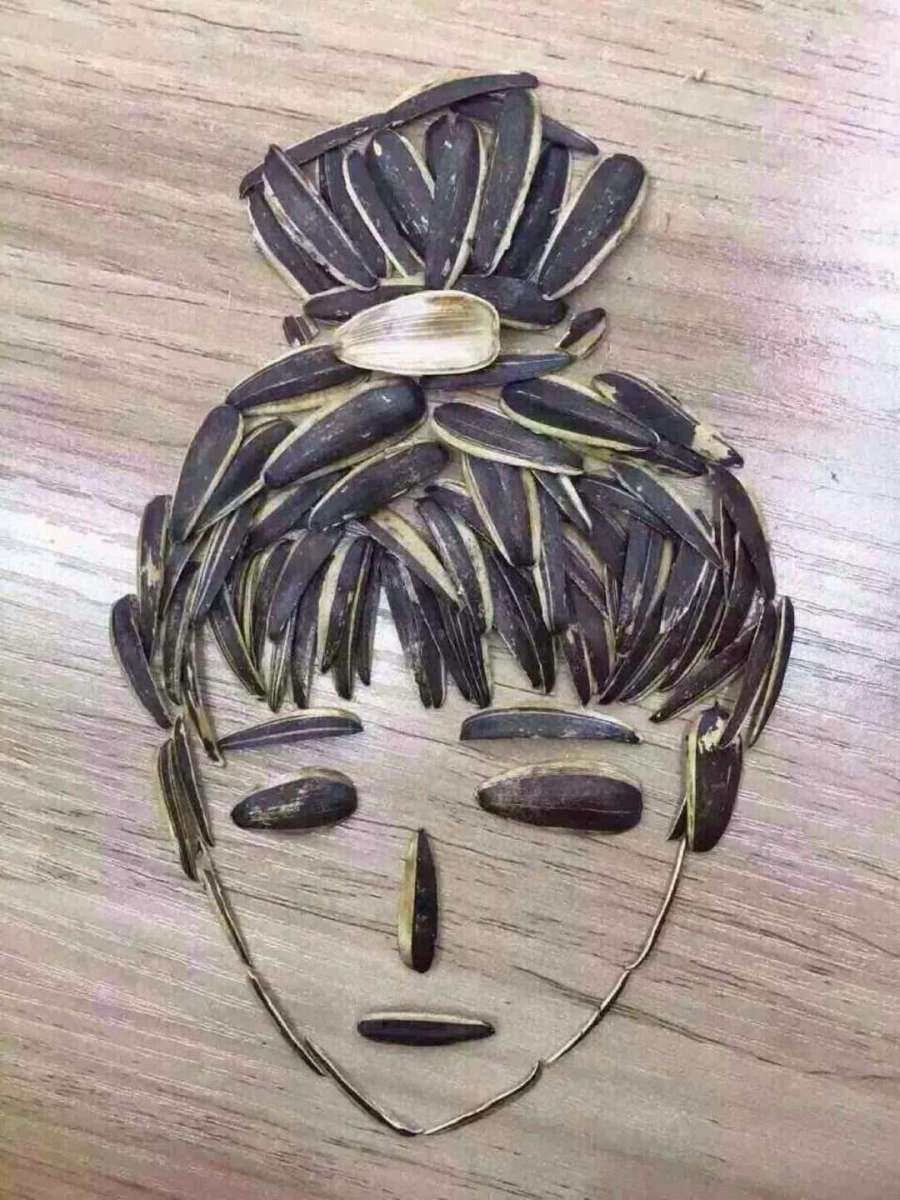
\includegraphics[height=3cm]{figure/test}
\caption{测试图片}
\label{fig:test}
\captionnote{这是个小图片. 该图片来自网络, 请勿用于商业用途.}
\end{figure}

\autoref{fig:test-big} 放在了浮动环境 \verb|figure| 中.
但由于占用空间较大, 它很有可能会跑到其他地方去了.

\begin{figure}[!htbp]
\centering
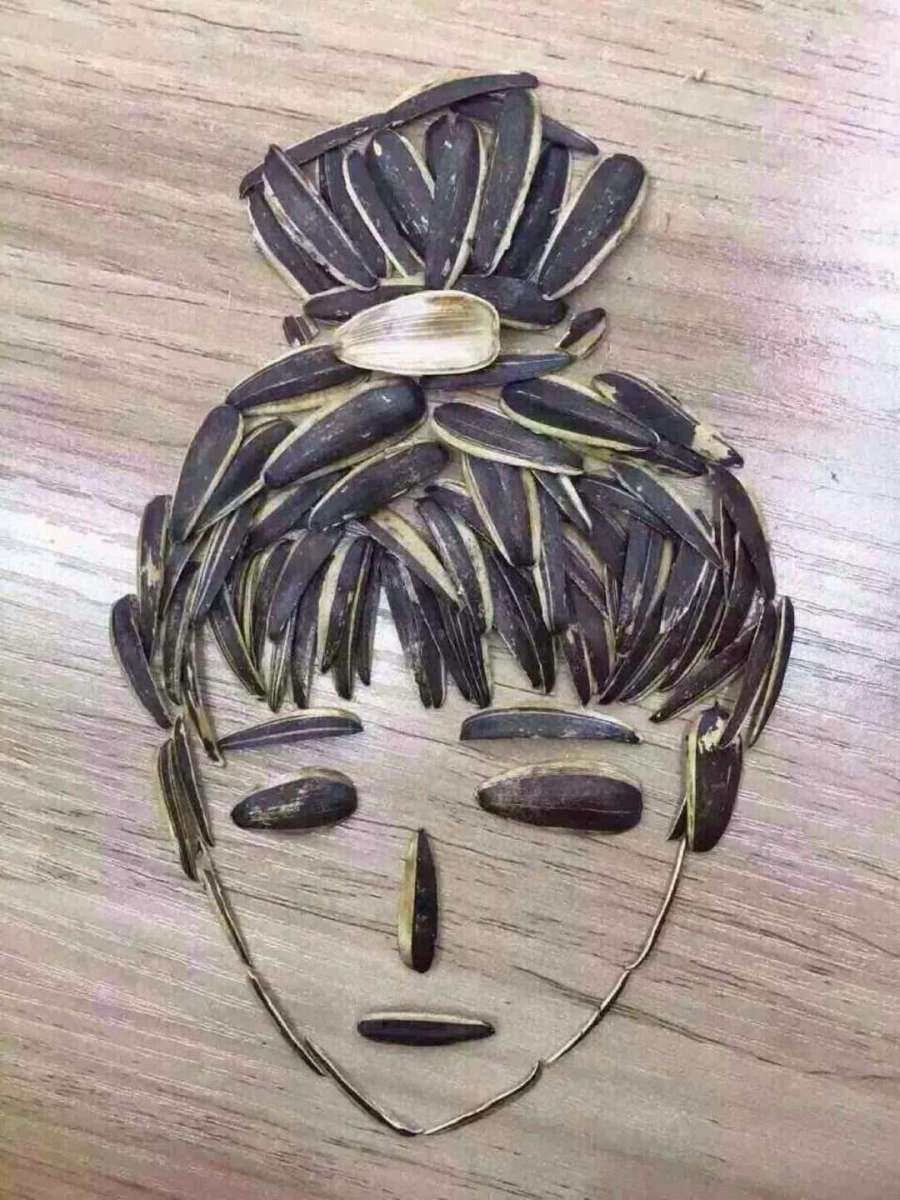
\includegraphics[width=8cm]{figure/test}
\caption{尺寸较大的图片}
\label{fig:test-big}
\captionnote{这是个尺寸较大的图片. 该图片放在了 \texttt{figure} 浮动环境中. 它的位置可以浮动. 它很有可能不会出现在代码所在的位置. 由于使用了 \texttt{p} 选项, 它很有可能独占了一页. 该图片来自网络, 请勿用于商业用途.}
\end{figure}

\subsection{表格}

\autoref{tab:test} 放在了浮动环境 \verb|table| 中.
由于占用空间很小, 它很有可能就在下面.

\begin{table}[!htb]
  \caption{普通表格}
  \label{tab:test}
  \centering
  \begin{tabular}{ccc}
    \toprule
    左 & 中 & 右\\
    \midrule
    1  & a  & b\\
    2  & a  & b\\
    3  & a  & b\\
    \bottomrule
  \end{tabular}
  \captionnote{这是个普通表格.}
\end{table}

\section{参考文献}
\label{sec:bib}

参考文献引用部分使用了 \verb|natbib| 宏包.
该宏包修改了 \verb|\cite| 命令, 并提供了新命令 \verb|\citet| 和 \verb|\citep|.

\verb|natbib| 宏包提供了两种引用模式: author-year 和 numerical.
它们可分别使用 \verb|authoryear| 和 \verb|numbers| 选项激活.
numerical 模式还有上标的形式, 可由 \verb|super| 选项激活.
其中 \verb|authoryear| 为默认选项.

宏包预定义了圆括号和方括号两种定界符, 分别使用 \verb|round| 和 \verb|square| 选项激活.
其中 \verb|round| 为默认选项.

本模板载入该宏包时使用了 \verb|numbers| 和 \verb|square| 选项.

命令 \verb|\bibliographystyle| 用于指定参考文献的样式. 它的参数是要使用参考文献样式对应的 \verb|.bst| 文件的文件名 (不包括扩展名). 宏包 \verb|natbib| 的作者提供了三个可用于 \verb|authoryear| 模式的 \verb|.bst| 文件: \verb|plainnat.bst|, \verb|abbrvnat.bst|, \verb|unsrtnat.bst|.

需要注意的是, 一些标准的 \verb|.bst| 文件 (如 \verb|plain.bst|) 只支持 numerical 模式.
在 author-year 模式下使用这些文件格式可能会遇到下述的错误信息.\\
\verb|Bibliography not compatible with author-year citations.|\\
此时只使用 numerical 模式即可.

如果使用的 \verb|.bst| 文件支持 author-year 模式,
在行文中是可以随时通过 \verb|\setcitestyle| 命令切换引用模式的.
\begin{itemize}
  \item
    \verb|\setcitestyle{authoryear,round}| 切换到 author-year 模式,
    并选定圆括号作为定界符.
  \item
    \verb|\setcitestyle{numbers,square}| 切换到 numerical 模式,
    并选定方括号作为定界符.
  \item
    \verb|\setcitestyle{super}| 切换到上标的 numerical 模式,
    不更改定界符.
\end{itemize}

研究生论文撰写手册要求, 对多作者的文献进行缩写时区分中英文文献的缩写词后缀. 这可能需要自己编写新的 \verb|.bst| 文件. 用户如有这样的要求的话, 可自行编写或下载满足条件的 \verb|.bst| 文件
\footnote{例如: \url{https://github.com/ustctug/gbt-7714-2015}}.

\subsection{numerical 模式}

命令 \verb|\setcitestyle{numbers,square}| 切换到 numerical 模式, 并选定方括号作为定界符.
此时三个引用命令的效果如下表所示.

\setcitestyle{numbers,square}
\begin{center}
  \begin{tabular}{ll}
    \toprule
    命令                      & 效果\\
    \midrule
    \verb|\cite{Knuth1986a}|  & \cite{Knuth1986a}\\
    \verb|\citet{Knuth1986a}| & \citet{Knuth1986a}\\
    \verb|\citep{Knuth1986a}| & \citep{Knuth1986a}\\
    \bottomrule
  \end{tabular}
\end{center}

在 \verb|natbib| 宏包中, 这些引用命令都有两个可选参数, 分别是引用的前缀和后缀.
例如, 命令 \verb|\cite| 在 \verb|numbers| 模式下的效果如下.\\
\verb|\cite[参见][第~1~章]{Knuth1986a}|
$\Rightarrow$
\cite[参见][第~1~章]{Knuth1986a}

\subsection{上标的 numerical 模式}

命令 \verb|\setcitestyle{super}| 切换到上标的 numerical 模式, 不更改定界符.
此时三个引用命令的效果如下表所示.

\setcitestyle{super}
\begin{center}
  \begin{tabular}{ll}
    \toprule
    命令                      & 效果\\
    \midrule
    \verb|\cite{Knuth1986a}|  & \cite{Knuth1986a}\\
    \verb|\citet{Knuth1986a}| & \citet{Knuth1986a}\\
    \verb|\citep{Knuth1986a}| & \citep{Knuth1986a}\\
    \bottomrule
  \end{tabular}
\end{center}

\subsection{author-year 模式}

命令 \verb|\setcitestyle{authoryear,round}| 切换到 author-year 模式, 并选定圆括号作为定界符.
此时三个引用命令的效果如下表所示.

\setcitestyle{authoryear,round}
\begin{center}
  \begin{tabular}{ll}
    \toprule
    命令                      & 效果\\
    \midrule
    \verb|\cite{Knuth1986a}|  & \cite{Knuth1986a}\\
    \verb|\citet{Knuth1986a}| & \citet{Knuth1986a}\\
    \verb|\citep{Knuth1986a}| & \citep{Knuth1986a}\\
    \bottomrule
  \end{tabular}
\end{center}

引用命令在 author-year 模式下会对多作者的文献使用 ``author1 et al.'' 的形式进行缩写.
而带星号的引用命令则会罗列所有作者. 这些命令也都可以一次引用多个文献.
使用效果参见\autoref{tab:cite-multi-author}.

\begin{table}[!htb]
  \caption{文献引用效果}
  \label{tab:cite-multi-author}
  \centering
  \begin{tabular}{lp{0.45\textwidth}l}
    \toprule
    命令                                   & 效果\\
    \midrule
    \verb|\cite{Mittelbach2004}|           & \cite{Mittelbach2004}\\
    \verb|\cite*{Mittelbach2004}|          & \cite*{Mittelbach2004}\\
    \verb|\cite{Knuth1984,Knuth1986a}|     & \cite{Knuth1984,Knuth1986a}\\
    \verb|\cite{Knuth1984,Mittelbach2004}| & \cite{Knuth1984,Mittelbach2004}\\
    \verb|\cite{Liu2013,Deng2001}|         & \cite{Liu2013,Deng2001}\\
    \bottomrule
  \end{tabular}
\end{table}

我们指出以下两点注意事项.
\begin{itemize}
  \item
    如果行文中使用了 author-year 模式, 则在 \verb|\bibliography| 命令之前应该切换回 numerical 模式. 否则参考文献列表前面不会有数字编号的前缀.
  \item
    如果使用了 \verb|.bib| 文件生成参考文献列表, 则列表中的每一条文献都需要在正文中使用 \verb|\cite| 等命令引用. 否则应该使用命令 \verb|\nocite| 声明.
\end{itemize}
